\section{Introduction}

A verifier can reject a proposed answer without telling a model how to find a better one. This distinction matters when evaluating systems that revise their own outputs or pass an unfinished solution to another model. An apparent improvement can come from additional samples, another opportunity to revise, a useful counterexample, or a stronger model receiving the final turn. These mechanisms require different controls. Agreement among models supplies none of the guarantees of an executable specification.

We study these distinctions in two small domains where correctness is completely checkable: finding a directed path and synthesizing a Boolean expression from its full truth table. The domains deliberately remove uncertainty about answer evaluation. They also have efficient classical solutions, which we measure. The objective is to examine the behavior of model-based proposal and revision procedures, not to show that language models are needed to solve these tasks.

The original experiment compares three-call independent sampling, revision with only a validity flag, and revision with exact checker feedback. Each homogeneous strategy selects its model on a separate development panel. Two further controls use one call from each of three configured models, either independently or as a serial feedback trajectory. All methods have the same call count and completion-token cap. Token use and observed latency remain outcomes, rather than being assumed equal. A separate exact solver establishes the performance available from the public problem specification.

The original study uses 48 development tasks and 256 test tasks, with fixed allocation across two families and three grades. A development gate checks that each family has an intermediate-performance region before test inference begins. The protocol, task manifest, selection rule, practical margin, and analysis code were frozen locally before the extension experiment. This was not a public preregistration. All scheduled observations were collected, and an independent analysis reconciled the raw responses, certificates, portfolio memberships, costs, and source fingerprints.

In the original study, exact-feedback refinement solved 117 of 256 test tasks. Validity-only refinement solved 115, and independent sampling solved 78. The mixed-model refinement solved 106. Neither prespecified conservative interval establishes the required five-percentage-point advantage of exact feedback over both homogeneous controls. In addition, a serving abort in one secondary mixed-model trajectory activates the protocol's global exclusion rule. The main result is therefore a diagnostic comparison, not a confirmed superiority claim. The primary homogeneous trajectories contain no serving errors, and the interval criterion would still fail without that exclusion.

A post-study follow-up replaced Llama with Mistral throughout development and testing, collecting fresh responses from all retained configurations on the same task panel. It completed without serving errors. Development selected Mistral for sampling and validity feedback, but Gemma for exact feedback. The larger cross-configuration feedback contrast shrank substantially when compared with the same-Gemma validity control. This follow-up is descriptive because it reuses previously examined tasks; it neither replaces the original study nor supplies independent confirmation.

The contribution is an auditable comparison of revision, feedback detail, and model mixing under strong local controls. Both studies retain task-family floors, ceilings, and operational outcomes that an aggregate improvement would conceal.

\section{Related Work}

Repeated generation is a substantive baseline. Self-consistency samples reasoning paths and aggregates their answers~\cite{wang2023selfconsistency}. Our independent control instead accepts any candidate that passes an exact checker; it does not reproduce chain-of-thought prompting or majority voting. Budget-aware evaluations also show why sophisticated inference procedures should be compared with simple alternatives at comparable resource allocations~\cite{wang2024tokeneconomies}. We match calls and completion caps while recording the remaining resource differences.

Self-Refine studies iterative generation and self-generated feedback~\cite{madaan2023selfrefine}. Reflexion uses feedback and linguistic memory across attempts~\cite{shinn2023reflexion}. Both precede the present experiment. Our contribution is not the idea of iterative correction. We restrict the history to the immediately previous candidate and contrast a binary validity message with an exact external diagnostic. Work on intrinsic self-correction finds important limitations when external feedback is absent~\cite{huang2024selfcorrect}; those findings do not establish that executable counterexamples are ineffective.

Multi-agent debate supplies another route to improved reasoning~\cite{du2024debate}. Evaluations questioning weak debate baselines and emphasizing model heterogeneity already motivate strong homogeneous comparisons~\cite{zhang2025overvaluing}. More directly, Zhao et al. distinguish the supply of useful proposals from verification-aware selection and study matched-budget interventions~\cite{zhao2026debate}. Thus, complementarity, verifier-sensitive selection, and budget matching are established research questions. The present study contributes a small exact-checker setting with a validity-only revision control, development-selected local configurations, complete candidate accounting, and explicitly retained adverse evidence. Its serial handoff is not a reimplementation of those full debate systems.

Counterexample-guided synthesis has a longer history of alternating candidate construction and verification~\cite{solarlezama2008sketching}. Replacing the synthesizer with a pretrained model does not make that loop new. Likewise, grammar-constrained decoding can enforce output syntax~\cite{park2025grammar}. This experiment uses strict parsing after unconstrained generation, not grammar-constrained decoding. Syntactic failures therefore remain part of the measured system behavior. We separate them from semantically incorrect, well-formed certificates, rather than interpreting every rejected output as a reasoning failure.

\section{Original Task Panel and Experimental Separation}
\label{sec:tasks}

\subsection{Directed-path construction}

Each graph is a layered directed acyclic graph. The initial layer contains one node. A construction procedure plants a path through successive layers and independently adds other forward edges between adjacent layers with probability 0.28. The input contains a shuffled edge list, a start node, a goal node, and a maximum path length. Node names are randomly assigned labels; the layer partition and planted construction path are not supplied.

The requested certificate is a JSON object containing a node sequence. The checker verifies types, the specified endpoints, the length limit, and every directed edge. A disconnected pair in the sequence or an incorrect endpoint is sufficient for rejection. Because a path is planted, every generated task has at least one solution. Grade changes increase both depth and width (Table~\ref{tab:tasks}); they do not isolate either factor's causal effect.

\subsection{Boolean-program synthesis}

Each Boolean task supplies the complete truth table of a generated function, in lexicographic input order. A candidate must be a JSON object with exactly one expression field. Its abstract syntax tree permits Boolean constants, the named variables, unary \texttt{not}, and binary \texttt{and}, \texttt{or}, and \texttt{xor}. Trees may contain at most 127 nodes and have depth at most 12. The checker interprets this restricted language directly; it does not execute arbitrary model-generated code.

The generator recursively samples expressions using the permitted operators. A leaf selects a variable and may negate it. Internal nodes select unary negation or a binary operator; an early-leaf option allows shorter expressions. We retain only functions in which every declared variable is essential and the truth table has at least two zeros and two ones. The lowest grade uses three variables; the others use four. Generating depth is a property of the sampled construction, not the shortest possible expression for its function. Distinct expression trees may implement the same function.

All $2^v$ assignments are checked, so acceptance establishes semantic equivalence to the supplied table within this finite language. For a well-formed but incorrect expression, the exact-feedback condition returns the first failing assignment, the proposed output, and the required output. For malformed expressions it returns the relevant syntax diagnostic. Truncated, unfinished, or unparsable responses are failures. The parser rejects duplicate JSON keys and extra text rather than silently extracting a favorable answer.

\begin{table}[t]
\caption{Fixed task grades and allocation. Each row has eight development tasks. Depth is graph depth or Boolean generating depth, not minimal solution complexity.}
\label{tab:tasks}
\centering\small
\begin{tabular}{llrrr}
\toprule
Family & Grade & Depth & Width / vars. & Test $n$\\
\midrule
Graph & 0 & 4 & 3 & 43\\
Graph & 1 & 7 & 5 & 43\\
Graph & 2 & 10 & 6 & 42\\
Boolean & 0 & 2 & 3 & 43\\
Boolean & 1 & 3 & 4 & 43\\
Boolean & 2 & 4 & 4 & 42\\
\bottomrule
\end{tabular}
\end{table}

\subsection{Development, test, and prior observations}

The manifest contains two separate format demonstrations, 48 development tasks, and 256 test tasks. The same family-specific demonstration is included in every condition. All 306 entries have distinct stored semantic signatures. Boolean functions are deduplicated by complete truth table within variable arity. Graph signatures canonicalize construction indices; they do not identify every graph isomorphism. The manifest also excludes signatures from the earlier full and smoke experiments and the extension smoke panel.

This separation prevents direct reuse of known generated instances. It does not establish absence from model pretraining, nor does it turn the grades into a clean out-of-distribution test. The models' training corpora are not known. The finite accepted generator, including exclusions and rejection rules, defines the population to which a cautious sampling interpretation could apply.

An earlier 48-test-task pilot exposed a graph ceiling and a Boolean floor. Those observations motivated the present prospective grading and development gate. We do not pool its outcomes with this test panel. A separate retrospective audit examined 720 old candidate outputs. Eight complete expressions admitted a narrowly defined reassociation of n-ary associative operators into binary trees; none became a correct certificate. No missing tokens were added and no operators or values were changed. Original scores remained unchanged. This diagnostic tests one specific representation issue, not every possible formatting intervention.

\section{Models, Strategies, and Resource Accounting}
\label{sec:methods}

\subsection{Original configured systems}

The original study evaluated three installed model configurations through Ollama 0.40.13 on an Apple ARM64 laptop with 128~GiB of memory and 18 CPU cores. Table~\ref{tab:models} gives the local tags, recorded runner metadata, and digest prefixes. Sizes embedded in tags are identifiers, not independently verified parameter counts. Training exposure and tokenization are not controlled; recorded quantization and execution backends also differ. The experiment therefore compares these configured systems, not architecture families under controlled training.

Every request explicitly used temperature 0.7, top-$p$ 0.9, repetition penalty 1.0, an 8,192-token context, a 512-token completion cap, and a recorded seed. Thinking was disabled where the server reported that capability. Other model-specific defaults were retained. Prompts request a single certificate and use the same public task data. There is no fine-tuning, parameter update, learned router, persistent memory, or external tool call by the model. Task and strategy order are deterministically shuffled to reduce simple ordering artifacts, but timing is not an isolated performance benchmark.

\begin{table}[t]
\caption{Original installed configurations. Full digests and server metadata are preserved in the artifact. A dash means the metadata field was not reported.}
\label{tab:models}
\centering\small
\begin{tabular}{llll}
\toprule
Local tag & Runner & Quant. & Digest prefix\\
\midrule
\texttt{qwen3.5:4b} & MLX & nvfp4 & \texttt{7f3251fa6878}\\
\texttt{llama3.1:8b} & GGML & Q4\_K\_M & \texttt{46e0c10c039e}\\
\texttt{gemma4:12b} & MLX & --- & \texttt{c7597fc90b86}\\
\bottomrule
\end{tabular}
\end{table}

\subsection{Strategy families and matched controls}

\textbf{Independent sampling (I).} A single configuration receives three fresh requests for the same task. Each request contains the format demonstration and public problem, with a distinct recorded seed. No generated candidate is supplied to another call.

\textbf{Validity-only refinement (V).} The first request is shared with the corresponding independent portfolio. Each of two subsequent calls receives the previous candidate and only its \texttt{VALID} or \texttt{INVALID} verdict, together with a request to revise. A valid candidate may be preserved. The model sees its previous answer, so comparison with independent sampling measures the entire revision procedure, not the validity bit alone.

\textbf{Exact-feedback refinement (E).} The call structure matches V, but the feedback additionally reports an invalid edge, endpoint error, syntax diagnostic, or Boolean counterexample. V and E share the initial candidate and use the same declared seed at each revision position. Only the immediately previous candidate is included, as quoted data. This comparison is the most direct test of the additional diagnostic information under the chosen prompting procedure.

\textbf{Mixed independent sampling (MI).} One independent candidate is drawn from each of the three configurations. \textbf{Mixed exact-feedback refinement (ME)} instead passes the previous candidate and exact feedback through a fixed three-model order. This is a serial handoff, not a voting rule or a general multi-agent debate protocol.

Every portfolio schedules all three calls, even after a valid certificate has appeared. Its outcome is
\begin{equation}
Y_{im}=\mathbf{1}\{\text{at least one of the three candidates passes}\},
\label{eq:outcome}
\end{equation}
for task $i$ and method $m$. Thus, a correct early answer survives a later unsuccessful revision. No majority vote or learned judge selects the answer. The exact verifier supplies the common acceptance rule.

\subsection{Selection and feasibility gate}

Development evaluates I, V, and E separately for every configuration. Each strategy selects the configuration with the largest development solve count, breaking ties by the declared model order. The mixed refinement order sorts configurations by development E count, then I count, then declared order. These choices are frozen before test inference. We also retain I and V controls for E's selected configuration in case the strongest baseline selections differ. They select the same configuration in the original study, so these additional labels duplicate original trajectories. The follow-up in Section~\ref{sec:replacement} selects different configurations, making the matched controls distinct.

The development gate requires no request errors, at least half of candidate outputs to be syntactically well formed in each family, and an intermediate-performance cell in each family. The last condition means that at least one prespecified selected strategy must solve between one and seven of eight tasks in at least one grade of that family. A failed gate would preserve diagnostics and skip test inference. Passing does not permit dropping easy or difficult test grades. All six strata remain in the primary denominator.

\subsection{Costs and classical baselines}

The experiment distinguishes physical requests from counterfactual portfolio cost. Reused initial candidates and independent samples are generated once, but their full cost is charged to every strategy that uses them. Development requires seven physical calls per configuration and task: three independent candidates plus two revisions for each feedback condition. Test execution reuses the selected configurations' calls wherever possible. This reuse improves efficiency and preserves pairing; it does not create independent replications.

Matching three calls and their completion caps does not match prompt length, emitted tokens, FLOPs, or latency. We retain prompt and output tokens, request wall time, available backend timing, model loading, and checker time. Missing usage from an aborted request is not treated as zero. Portfolio timing is the sum of charged observations, not a measured standalone replay of each strategy with controlled cache state.

Two public-input algorithms provide exact baselines. Breadth-first search finds a graph path. For Boolean synthesis, a balanced disjunctive normal form represents the smaller truth-table class, using an outer negation when appropriate. These expressions satisfy the checker limits. Their certificates never enter test prompts. Both methods solve the actual supplied problem without consulting a stored reference answer. Their timing includes proposal construction and verification, and is reported separately from model-server latency.

\section{Original Prespecified Analysis}
\label{sec:analysis}

The experimental unit is a task instance with paired strategy outcomes. The primary estimand is the difference in solve probability for E versus each of the development-selected I and V baselines, weighted by the fixed six-stratum allocation. We do not treat individual candidates, model turns, duplicate control labels, or the three configurations as independent experimental replications.

For baseline $b$, let $D_i=Y_{iE}-Y_{ib}$ and define positive and negative discordance probabilities $p_s^+=\Pr(D_i=1\mid s)$ and $p_s^-=\Pr(D_i=-1\mid s)$ in stratum $s$. With $w_s=n_s/256$, the target is
\begin{equation}
\Delta_b=\sum_{s=1}^{6} w_s(p_s^+-p_s^-).
\end{equation}
The empirical estimate is the paired mean over the 256 fixed tasks. For each comparison, the frozen analysis constructs Clopper--Pearson binomial limits~\cite{clopper1934limits} for both discordance probabilities in every stratum. It allocates tail probability $\alpha/(4S)$ with $\alpha=0.025$ and $S=6$. If these limits are $[L_s^+,U_s^+]$ and $[L_s^-,U_s^-]$, the difference interval is
\begin{equation}
\left[\sum_s w_s(L_s^+-U_s^-),\;\sum_s w_s(U_s^+-L_s^-)\right].
\label{eq:interval}
\end{equation}

The union construction gives at least 97.5\% coverage per comparison and at least 95\% jointly for the two primary comparisons under independent binomial sampling within strata. Semantic deduplication and finite generator support make that sampling model a working approximation, not a distribution-free guarantee. The bounds are deliberately conservative. In particular, strata with zero observed discordance retain nonzero uncertainty. We preserve this rule rather than replacing it after inspection with a narrower test.

The practical superiority criterion requires \emph{both} lower limits to exceed $0.05$. An interval crossing that margin leaves the corresponding claim unresolved. Failure to meet the criterion is neither an equivalence finding nor evidence that the effect is exactly zero. Mixed-model comparisons, individual strata, costs, and the reused first-call reference are descriptive secondary analyses.

The protocol also specifies that any request error prevents scientific superiority inference. Wrong, malformed, truncated, and unfinished candidates remain observed failures, while serving errors are separately classified and retain their measured wall cost. An interrupted schedule would leave missing observations missing. This strict operational gate applies globally, including secondary trajectories. We report the planned intervals even when the gate is triggered, but do not reinterpret them as an eligible confirmatory analysis.

\section{Original Frozen-Study Results}
\label{sec:results}

\subsection{Development selection and gate}

Development solve counts for I, V, and E were respectively 12, 12, and 10 for \texttt{qwen3.5:4b}; 6, 3, and 5 for \texttt{llama3.1:8b}; and 15, 19, and 20 for \texttt{gemma4:12b}, each out of 48. All three homogeneous selections therefore chose Gemma. The mixed refinement order was Gemma, Qwen, then Llama. The matched I and V controls coincide exactly with the selected baselines and are not additional evidence.

The gate passed, but only weakly for Boolean tasks. Graph grade 0 was already at ceiling for all selected strategies. Grades 1 and 2 contained intermediate cells. Boolean grade 0 had development counts of 0, 1, and 1 for I, V, and E; grades 1 and 2 were zero for all three. Well-formed candidate counts were 404/504 for graphs and 265/504 for Boolean tasks. These met the frozen threshold. The test panel was then evaluated in full, without removing anticipated floor cells.

\subsection{Aggregate outcomes and primary comparisons}

Table~\ref{tab:outcomes} reports the five unique three-call methods and two distinct-budget references. E solved 117 tasks, V solved 115, and I solved 78. The observed E--I difference is 39/256, or 15.23 percentage points. All 39 discordant tasks favored E. The conservative interval is nevertheless $[-8.14,34.46]$ percentage points because of the prespecified stratum-wise construction. E--V has four favorable and two unfavorable discordant tasks, giving a difference of 0.78 points and interval $[-16.44,18.01]$. Neither lower limit exceeds five points (Figure~\ref{fig:primary}).

\begin{table}[t]
\caption{Original test outcomes. All rows use the same 256 tasks. The one-call row reuses an existing candidate and is secondary; the exact solver has a different computational procedure. Duplicate matched-control labels are omitted.}
\label{tab:outcomes}
\centering\small
\begin{tabular}{lrrr}
\toprule
Method & Calls & Solved & Rate (\%)\\
\midrule
Independent (I) & 3 & 78 & 30.47\\
Validity feedback (V) & 3 & 115 & 44.92\\
Exact feedback (E) & 3 & 117 & 45.70\\
Mixed independent (MI) & 3 & 88 & 34.38\\
Mixed exact feedback (ME) & 3 & 106 & 41.41\\
\midrule
Reused first call & 1 & 74 & 28.91\\
Public-input exact solver & 0 & 256 & 100.00\\
\bottomrule
\end{tabular}
\end{table}

\begin{figure*}[t]
\centering
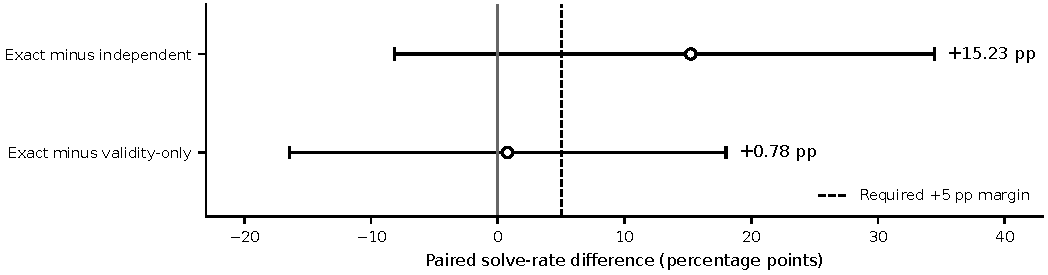
\includegraphics[width=\textwidth]{figures/topic3_primary_comparisons.pdf}
\caption{Original prespecified paired differences and conservative 97.5\% intervals. The five-point margin must be exceeded by both lower bounds. Neither comparison passes. The intervals retain the frozen analysis despite the study's separate global serving-error exclusion; they are not a repaired confirmatory result.}
\Description{Two horizontal confidence intervals compare exact feedback with independent sampling and validity feedback. Both cross zero and the five-percentage-point threshold.}
\label{fig:primary}
\end{figure*}

V improves on I by an observed 37 solves, while E adds two further solves in the aggregate. This decomposition is more informative than reporting E against fresh sampling alone. It does not establish that a binary validity bit caused the larger difference: V also supplies the previous candidate and a revision instruction. Nor does the small E--V estimate establish equivalence, given the wide interval.

MI solved 88 tasks, ten more than homogeneous I. ME solved 106, eighteen more than MI but eleven fewer than homogeneous E. These are descriptive comparisons for a fixed local pool and order. They do not establish a general diversity benefit or a population-level disadvantage of collaboration. The secondary first-call reference solved 74 tasks; its additional independent samples raised the selected independent portfolio to 78. Because that reference reuses an existing response and uses one call, it is not a separate matched-budget strategy.

\subsection{Family and grade structure}

Table~\ref{tab:strata} shows the mechanism's uneven operating region. E solved 112/128 graph tasks and 5/128 Boolean tasks. V also solved 112 graph tasks, with only three Boolean successes. On graph grade 2, both feedback methods solved 32/42 tasks versus 8/42 for I. On the easiest graph grade, almost every method was near ceiling. Boolean grade 1 remained at zero across every strategy; grade 2 had one E success and none for the other four methods.

\begin{table}[t]
\caption{Original solved tasks by fixed family and grade. Columns abbreviate the five strategies defined in Section~\ref{sec:methods}. Counts, rather than candidate-level rates, preserve the task as the experimental unit.}
\label{tab:strata}
\centering\small
\begin{tabular}{llrrrrrr}
\toprule
Family & Grade & $n$ & I & V & E & MI & ME\\
\midrule
Graph & 0 & 43 & 41 & 42 & 42 & 43 & 42\\
Graph & 1 & 43 & 28 & 38 & 38 & 30 & 34\\
Graph & 2 & 42 & 8 & 32 & 32 & 13 & 29\\
Boolean & 0 & 43 & 1 & 3 & 4 & 2 & 1\\
Boolean & 1 & 43 & 0 & 0 & 0 & 0 & 0\\
Boolean & 2 & 42 & 0 & 0 & 1 & 0 & 0\\
\bottomrule
\end{tabular}
\end{table}

The development gate therefore did not produce broadly informative Boolean comparisons. It identified a narrow intermediate cell but allowed a test panel dominated by failures in that family. This is an important design limitation, not a reason to discard the difficult cells after observing them. Aggregate differences largely reflect graph behavior. The lone grade-2 Boolean success also cautions against reading generating depth as a monotone semantic difficulty scale.

\subsection{Candidate failures and the serving abort}

Across 2,816 physical test requests, the checker recorded 904 verified candidates, 728 Boolean counterexamples, 730 malformed responses, 226 truncations, 147 invalid-edge reports, 80 endpoint errors, and one serving error. Graph candidates accounted for 887 verified outputs; Boolean candidates accounted for 17. Boolean requests additionally produced 728 well-formed semantic failures, 539 malformed responses, and 123 truncations. These candidate counts diagnose failure modes. They are not 2,816 independent task observations and should not be substituted for the portfolio results.

The sole serving error occurred on the third call of ME for a grade-1 Boolean task. The Llama server returned HTTP 500 with a token-repeat-limit abort after 5.304 seconds. This was a local serving failure, not a network disconnect or a semantically checked answer. Only the mixed-feedback portfolio used that failed call. All primary Gemma portfolios were error-free. Nevertheless, the frozen global exclusion rule makes the scientific comparison ineligible.

The affected task failed under all five strategies. If the unobserved failed candidate were assumed correct, ME could increase only from 106 to 107 of 256; if incorrect, it remains 106. This secondary best/worst-case bound leaves the original counts intact and does not restore eligibility. It does not affect either primary comparison.

A separately documented post-study amendment repeated exactly the failed payload once, with the same model digest, server version, seed, and request options. It again ended in the token-repeat-limit abort, after 5.208 seconds. A further single-task diagnostic substituted \texttt{mistral-small3.2:24b}. That request completed, but its expression failed exact checking on input $(0,0,1,0)$, producing 1 where 0 was required. Neither diagnostic replaces an original response or enters the study denominator. The Mistral observation is not a cohort-wide model comparison.

\subsection{Resource use and the exact ceiling}

The original study made 3,824 physical calls: 1,008 in development and 2,816 in test. There were 3,823 completed responses, one request error, and no cache hits. Observed prompt tokens totaled 3,726,229 and output tokens 327,564, with both counts missing for the aborted call. All request wall times were observed, totaling 3,728.66 seconds. Recorded backend evaluation, prompt evaluation, and loading totaled 2,755.03, 929.34, and 18.56 seconds, respectively, each with one missing request. The stage elapsed approximately 62.4 minutes. The two later diagnostics are separate expenditures.

Figure~\ref{fig:cost} compares the observed quality and charged request wall time of the five distinct strategies. Mean wall cost per task was 4.346 seconds for I, 3.983 for V, 4.170 for E, 2.810 for MI, and 2.893 for ME. Feedback conditions sometimes emitted shorter responses, so additional prompt information did not translate monotonically into longer observed latency. Mixed portfolios used different configurations and backends. These measurements cannot establish an architectural efficiency advantage.

\begin{figure*}[t]
\centering
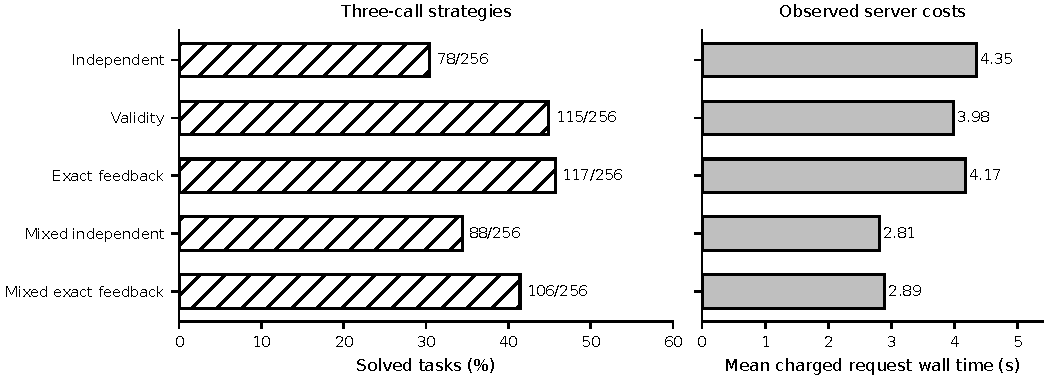
\includegraphics[width=\textwidth]{figures/topic3_quality_cost.pdf}
\caption{Original observed solve rates and mean charged request wall seconds for the five unique three-call strategies. Counts are over all 256 test tasks; wall time includes the failed request. Timing describes the observed laptop workload and shared-candidate accounting, including available loading costs and uncontrolled background activity. Equal calls and completion caps do not imply equal FLOPs or isolated latency.}
\Description{Aligned horizontal bar charts show solve rates and mean charged request wall time. Homogeneous exact feedback has the highest observed solve count, while mixed strategies have shorter observed wall times.}
\label{fig:cost}
\end{figure*}

Mean charged prompt/output tokens were 2,840/424 for I, 3,183/319 for V, 3,226/365 for E, and 2,579/223 for MI. For ME the available-case means were 2,866/217 over 255 complete portfolios; its failed portfolio is not assigned zero token cost. Wall means retain all 256 portfolios. Checker time was approximately 0.12--0.15 milliseconds per three-call portfolio.

The public-input exact algorithms solved all 256 tasks. Mean proposal time was 3.90 microseconds, and mean verification time was 38.29 microseconds. These small CPU measurements describe this implementation and task scale; they are not a hardware-normalized comparison with a model server. Even so, the existence of cheap exact algorithms decisively limits practical claims. The model results concern a proposal-and-feedback mechanism on finite tasks, not superiority over the strongest available solver.

\section{Full-Panel Model-Substitution Follow-Up}
\label{sec:replacement}

\subsection{Separate protocol and selection}

Following the original serving abort and the one-task diagnostics, we defined a full follow-up replacing \texttt{llama3.1:8b} with \texttt{mistral-small3.2:24b}. The latter used a GGML runner, recorded Q4\_K\_M quantization, and model digest prefix \texttt{5a408ab55df5}. Qwen and Gemma retained their original digests, and the server version was unchanged. All three configurations received fresh requests in a new response cache. No original response was imported.

The follow-up reused the identical 48 development and 256 test tasks, prompt templates, verifier, call caps, and model-selection rules. Actual revision prompts depended on the newly generated previous candidates. Its amendment was frozen before new inference. The development gate was recorded but declared non-stopping so the entire panel would be collected even if the gate failed. All comparisons were designated descriptive because the panel had already been examined. The gate passed, and all 4,848 scheduled physical requests completed without serving errors or response-cache hits. The original observations and exclusion decision remain unchanged.

Development I/V/E counts were 10/11/9 for Qwen, 17/18/16 for Mistral, and 14/18/19 for Gemma, each out of 48. Mistral therefore supplied the selected I and V baselines; its validity tie with Gemma was resolved by the declared order. Gemma supplied E. The mixed sequence became Gemma, Mistral, then Qwen. Unlike the original study, all seven allocations were distinct: the selected baselines and Gemma's matched controls could not be collapsed.

\subsection{Outcomes, controls, and costs}

Table~\ref{tab:replacement} reports every allocation. Gemma E solved 115 tasks, compared with 96 for Mistral I and 88 for Mistral V. The retained primary-form differences were 7.42 percentage points with a 97.5\% interval of $[-15.97,28.72]$, and 10.55 points with interval $[-14.85,32.88]$, respectively. Neither lower bound exceeded five points. These remain descriptive bounds, not a second eligible primary analysis.

\begin{table}[t]
\caption{Separate model-substitution follow-up. Each row uses three calls on the same 256 tasks. G and B count solves among 128 graph and 128 Boolean tasks; $s$ is mean charged request wall seconds. Timing remains descriptive.}
\label{tab:replacement}
\centering\small\setlength{\tabcolsep}{3pt}
\begin{tabular}{lrrrr}
\toprule
Allocation & G & B & Total & $s$\\
\midrule
Mistral independent & 90 & 6 & 96 & 6.167\\
Mistral validity & 84 & 4 & 88 & 6.557\\
Gemma exact feedback & 112 & 3 & 115 & 4.151\\
Mixed independent & 92 & 3 & 95 & 4.718\\
Mixed exact feedback & 109 & 2 & 111 & 4.754\\
Gemma independent control & 79 & 2 & 81 & 4.342\\
Gemma validity control & 110 & 1 & 111 & 3.769\\
\bottomrule
\end{tabular}
\end{table}

The same-configuration controls change the interpretation. Gemma's validity portfolio solved 111 tasks, leaving an E--V difference of only four tasks, or 1.56 points, with a descriptive 95\% interval of $[-14.89,17.67]$. The 27-task difference against selected Mistral V therefore cannot be attributed to feedback detail alone. Gemma E exceeded its matched independent control by 34 tasks, or 13.28 points, with interval $[-8.22,31.30]$. The selection rule was not revised after observing that Gemma V outperformed selected Mistral V on test. Mistral V also solved fewer tasks than Mistral I, so revision was not uniformly beneficial across configurations.

Mixed refinement solved 111 tasks, below Gemma E's 115; mixed independent sampling solved 95, compared with Mistral I's 96. The secondary reused Mistral first call solved 73. Boolean performance remained near floor: no allocation solved a grade-1 Boolean task, and at most two grade-2 tasks were solved by any allocation. The unchanged exact baseline solves all 256 identical tasks; its previously reported timing is not a new measurement in this follow-up.

The run comprised 1,008 development and 3,840 test calls. Selection differences required 15 distinct physical calls per test task, while each logical portfolio retained its three-call cap. Recorded usage was 4,942,530 prompt tokens and 369,437 output tokens, with no missing usage fields. Request wall times summed to 7,151.48 seconds; stage elapsed time was approximately 119.4 minutes. The follow-up used both different configurations and more distinct physical calls than the original experiment. These totals are not a matched-work estimate of the cost of substituting one model.

\subsection{Exploratory repeatability of retained requests}

A post hoc audit matched requests across runs using the complete recorded payload, model digest, and server identity. Across development and test, all 1,312 independently prompted Qwen/Gemma requests found exact matches. Raw text agreed in 601 cases and verifier acceptance in 1,250. Among 599 feedback requests with matching prior-context payloads, text agreed in 534 and acceptance in 594. The feedback subset is conditioned on identical contexts, and requests sharing a task are not independent task replications.

These observations show that fixed tags, digests, request options, and seeds did not ensure identical served outputs in this setup. They do not identify the cause of the variation. Consequently, aggregate changes between the two studies cannot be assigned solely to the model substitution. The follow-up supplies a separate configuration comparison with fresh responses, not an independent task sample or a repair of the original inference gate.

\section{Discussion and Limitations}

\subsection{What the comparisons establish}

In the original study, the central observation is the separation between the two feedback comparisons. Exact-feedback refinement has substantially more observed successes than fresh independent sampling, yet nearly the same total as validity-only refinement. Evaluating only the first contrast would attribute to detailed verification information an improvement also obtained by a simpler revision procedure. The second contrast supplies a necessary control, although its interval is too wide to resolve a small effect.

Original mixed independent sampling provides some additional verified coverage compared with the selected homogeneous independent portfolio. Serial cross-model feedback does not convert that coverage into an observed advantage over the strongest homogeneous refinement. This may reflect unequal model capabilities, an unhelpful handoff order, shared blind spots, prompt sensitivity, or the small call budget. The experiment cannot distinguish those explanations. In particular, it does not manipulate architecture diversity independently of training data, scale, quantization, or backend.

The follow-up reinforces the need to distinguish model selection from feedback information. A larger difference against the development-selected validity baseline coexists with a four-task difference against the same-Gemma validity control. Its mixed procedures again fail to exceed the best observed homogeneous exact-feedback count, but their rankings and costs are specific to these configurations. Neither study establishes a general collaboration advantage or a general failure of collaboration.

The one-task failure diagnostics also separate three questions: whether the server returned a candidate, whether that candidate was well formed, and whether it was correct. Repeating the failed request did not produce a candidate. Substituting Mistral on that request produced a checkable but wrong expression. Treating either intervention as an automatic recovery would confuse operational completion with semantic success.

\subsection{What remains untested}

The task panel is intentionally narrow. Graphs have known finite structure and a guaranteed path. Boolean truth tables expose the whole target function. These are not open-ended proofs, scientific hypotheses, hidden-test programming tasks, or measures of discovery beyond a training cutoff. No learned abstraction, continual update, or improvement to model weights is tested. An exact checker removes one source of evaluation error without making the proposal problem representative of scientific discovery.

The panel also retains substantial ceilings and floors. The Boolean condition has too few successes to characterize feedback behavior reliably across its higher grades. Strict output checking combines format compliance and semantic ability at the system level. Grammar-constrained generation could remove some format failures, but that would define a different protocol and needs fresh development and test data. The unchanged retrospective normalization result cannot stand in for that experiment.

The four configurations form fixed convenience pools, with no repeated training or independently sampled architecture families. Each run records one seeded response per scheduled position; neither samples a population of deployments. Fixed seeds do not ensure identical served text. Timing includes shared execution context and background activity, and token counts are tokenizer-dependent.

The original conservative intervals and global request-error rule reduce the ability to establish superiority; changing them after observing results would change the analysis. The error-free follow-up remains descriptive because it reuses examined tasks. Future work should prespecify a more efficient paired procedure and operational-failure estimand, require a broader intermediate-performance region, separate syntax constraints from semantic feedback, and include no-message or sham-feedback controls for causal communication claims. Those changes require new observations.

\section{Reproducibility and Artifact Scope}

The accompanying release candidate keeps the original and replacement evidence separate, with the frozen task manifest, response records, portfolio memberships, checker and analysis source, task-construction specification, model and server metadata, selection decisions, development gates, resource ledgers, and analysis outputs. Its portable audit regenerates task-level verdicts and reconciles them with stored results before producing tables and figures. The artifact is private during preparation; no public release or external artifact evaluation is claimed here.

Source and data fingerprints distinguish the original extension from final analysis and later amendments. The original extension source digest begins \texttt{845d06f30456}; the replacement extension begins \texttt{4a1d60587099}; the shared checker begins \texttt{04ee69f54923}. Full SHA-256 values accompany the records. An independent analysis found no disagreements in certificates, memberships, selection, gate decisions, counts, cost means, or primary bounds. It also checked that protected source inputs had not changed. Audit code includes malformed-certificate, interval-boundary, missing-call, and duplicate-identifier checks.

Recomputing this paper's tables requires no new model calls. Reproducing generation is a distinct operation requiring the pinned local configurations, server behavior, and complete prompting/controller environment retained in the original execution archive. The portable repository audits the included evidence; it does not supply a turnkey generation rerun. Identical text is not guaranteed merely by matching a seed. Raw physical usage is kept separate from logical portfolio charges. The first-call secondary reference is explicitly a reused observation, and duplicate matched-control labels are identified. The original serving error, the one exact-payload retry, the one-task alternative-model diagnostic, and the full substitution follow-up each retain separate provenance. None silently fills a missing token field or changes an original verdict.

\section{Conclusion}

In the original study, exact-feedback refinement solved 117/256 tasks, versus 115 for validity-only refinement, 78 for independent sampling, and 106 for mixed refinement. Its superiority criterion was not met, and a serving abort separately excluded confirmation. A full model-substitution follow-up completed without errors on the same panel: Gemma exact feedback solved 115 tasks, selected Mistral validity solved 88, and matched Gemma validity solved 111. The smaller same-configuration contrast prevents attributing the larger cross-model difference to feedback alone. Mixed refinement solved 111, and exact classical algorithms solve every task. Both studies retain a substantial Boolean floor. The evidence supports careful separation of revision, diagnostic detail, model selection, served-output repeatability, and resource use before broader claims about verifier-guided collaboration.
